%%%%%%%%%%%%%%%%%%%%%%%%%%%%%%%%%%%%%%%%%%%%%%%%%%%%%%%%%%%%%%%%%%%%%%%%
%                                                                      %
% This program is free software; you can redistribute it and/or modify %
% it under the terms of the GNU General Public License as published by %
% the Free Software Foundation; either version 2 of the License, or    %
% (at your option) any later version.                                  %
%                                                                      %
% This program is distributed in the hope that it will be useful,      %
% but WITHOUT ANY WARRANTY; without even the implied warranty of       %
% MERCHANTABILITY or FITNESS FOR A PARTICULAR PURPOSE.  See the        %
% GNU General Public License for more details.                         %
%                                                                      %
% You should have received a copy of the GNU General Public License    %
% along with this program; if not, write to the Free Software          %
% Foundation, Inc., 51 Franklin St, Fifth Floor, Boston,               %
% MA  02110-1301  USA                                                  %
%                                                                      %
%%%%%%%%%%%%%%%%%%%%%%%%%%%%%%%%%%%%%%%%%%%%%%%%%%%%%%%%%%%%%%%%%%%%%%%%
%
%       $Id$
%


% TODO:
% 	* Ajouter un slides sur la livraison
%	* Forme des TPs à venir: pré requis/connaissances acquises
%	* Préparer le TDs sur Mercurial
%	* Ajouter un slide de présentation
%
\documentclass[handout]{beamer}

\usepackage[french]{babel}
\usepackage[utf8]{inputenc}
\usepackage{listings}
\usepackage{multicol}

% Use to get nice looking array ?
% \usepackage{array}
% \usepackage{color}
% \usepackage{colortbl}
% \usepackage{longtable}

\usetheme{Warsaw} 

\title{TP - Génie Logiciel (1)}
\subtitle{Construction et gestion de sources}

\author{Romain PELISSE}
\institute{ESME Sudria}
\date{\today}

\logo{
\includegraphics[scale=0.3]{../img/logo-cc.png}}

\begin{document}
	% Definition de l'affichage de l'ensemble des codes
	\definecolor{white}{rgb}{1,1,1}
	\definecolor{vert_commentaire}{rgb}{0.03, 0.45, 0}
	\definecolor{rouge_chaine}{rgb}{0.128, 0, 0}
	% Définition du langage Ant
	\lstdefinelanguage{ant}
	{
		morekeywords={name,default,basedir,value,property,depends},
		otherkeywords={<project,</project>,<target,/target>,<echo>,</echo>},
		sensitive=false,
		morecomment=[s]{<!--}{-->},
		morecomment=[s]{<?xml}{?>},
		morestring=[b][\color{red}]",
	}

	\lstset{
		language=ant, 
		backgroundcolor=\color{white}, 
		basicstyle=\small, 
		showstringspaces=false,
		stringstyle=\ttfamily,
		commentstyle=\color{vert_commentaire},
		keywordstyle=\color{blue}\bfseries\emph
	}

% end...
\frame{\titlepage}

\section[Agenda]{}
\begin{frame}
	\begin{multicols}{2}
		\tableofcontents
	\end{multicols}
\end{frame}

\section{Introduction}
\subsection{Gérer un projet logiciel code}
\begin{frame}
	\begin{block}{Autour d'un projet de développement...}
		\begin{itemize}
 			\item La procédure de \textbf{compilation} et d'\textit{éditions de liens}
			\item Gérer les \textit{dépendances} du projets.
			\item Disposer d'une \textbf{documentation} synchronisée avec la version
			\item Le \textbf{packaging}:
			\begin{itemize}
				\item format exécutable (elf, exe, .app)
				\item embarquer (ou non) les dépendances
				\item version
			\end{itemize}	
			\item ...
		\end{itemize}
	\end{block}
\end{frame}
\begin{frame}
	\begin{block}{Objectifs}
		\begin{itemize}
 			\item Pouvoir \textbf{reconstruire} le projet facilement
			\item \textbf{Abstraire l'environement} de développement (OS, IDE,...)
			\item Reproduire de manière exacte \textbf{une version}, conserver toutes les versions
			\item Automatisation de la \textbf{non-régression}
			\item Effectuer des tâches redondantes \textbf{contrôle qualité}, \textbf{documentation},...
			\item \textbf{Assurer une livraison} de bonne qualité
		\end{itemize}
	\end{block}	
\end{frame}
\subsection{Les outils du Génie Logiciel}
\begin{frame}
 	\begin{block}{Tout ceci requiert des outils !}
		\begin{figure}[hbtp]
			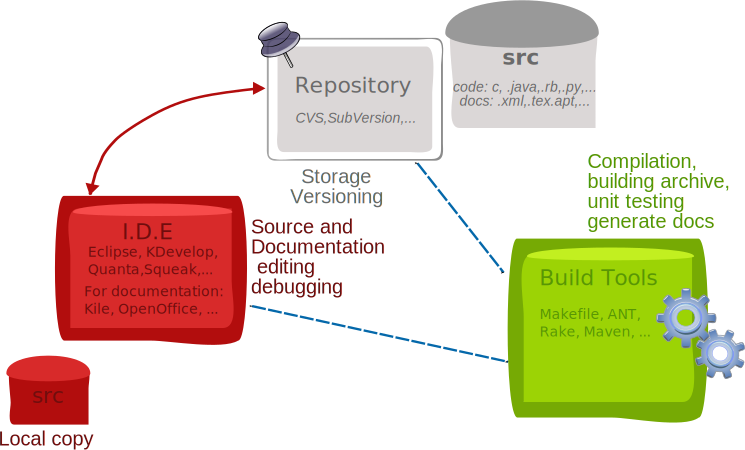
\includegraphics[scale=0.5]{../img/project-tools.png}
		\end{figure}
 	\end{block}
\end{frame}

\section{Outils de construction}
\subsection{Quel outil prendre et dans quel but ?}
\begin{frame}
 	\begin{block}{Objectif}
		\begin{itemize}
			\item Automatiser les tâches redondantes du projet:
				\begin{itemize}
					\item Exécution des tests unitaires
					\item Génération de la documentation
					\item Produire les artefacts
					\item ...
				\end{itemize}
			\item Permettre de facilement 'construire' le projet (compilation, packaging,...)
			\item Externaliser les paramètres (adresse IPs, paramètres par défaut,...)
			\item Automatiser les déploiements (serveur de pré-prod, prod)	
		\end{itemize}
	\end{block}
\end{frame}

\begin{frame}
	\begin{block}{Le nerf du projet : le build}
	 	Le \textbf{build} est donc un \underline{point essentiel du projet} car
		il est le seul garant de sa \textbf{maintenabilité}.
		\textit{Un projet sans build peut être impossible à reprendre, à maintenir ou à faire évoluer.}
	\end{block}
 	\begin{block}{La relation technologie/build}
		\begin{center}
			\begin{tabular}{|c|l|}
				\hline
				\textbf{Techno} & \textbf{Build} \\ 
				\hline
				OpenVMS & MMS  \\ 
				\hline
				C/C++ & CMake,\textbf{Makefile} \\ 
				\hline
				Java & \textbf{Ant}, Maven \\
				\hline
				C\# & NAnt \\
				\hline
				Ruby & Raven \\
				\hline 
			\end{tabular}
		\end{center}

% Improve the array ?
% 	\begin{center}
% 		% use packages: array,color,colortbl,longtable
% 		\newcommand{\mc}[3]{\multicolumn{#1}{#2}{#3}}
% 		\definecolor{tcA}{rgb}{0,0.5,0.5}
% 		\definecolor{tcB}{gray}{1}
% 		%
% 		\begin{longtable}[c]{lll}
% 		\rowcolor{tcA}
% 		\mc{1}{>{\columncolor{tcA}}l}{\color{tcB} } & \mc{1}{>{\columncolor{tcA}}l}{\color{tcB} ×} & \mc{1}{>{\columncolor{tcA}}l}{\color{tcB} ×} \\ 
% 		× & × & × \\ 
% 		× & × & × \\ 
% 		× & × & × \\ 
% 		× & × & × \\ 
% 		× & × & ×
% 		\end{longtable}
% 	\end{center}


 	\end{block}
\end{frame}



\subsection{Ant}
\begin{frame}
	\begin{block}{Historique du projet Ant}
		\begin{itemize}
			\item Outil de \underline{Build en Java}, alternative à Makefile:
				\begin{itemize}
				 	\item Trop complexe
					\item Peu adapté à Java
				\end{itemize}
			\item Fichier de description de tâche en XML
			\item Conçu en Java, donc portable sur tout les OS
			\item Appel : \texttt{ant} + série de tâches ( ex: \texttt{ant clean compile install} )
		\end{itemize}
	 \end{block}
\end{frame}



\begin{frame}
%\subsubsection{Structure d'un fichier de build Ant}
	\begin{block}{Structure du fichier}
			\begin{itemize}
				\item Tâche
				\item Interdépendance
			\end{itemize}
	\end{block}
	%TODO: Make a box !
	\lstinputlisting{../examples/syntax.xml}

\end{frame}

%\subsubsection{Fonctionnement}
\begin{frame}
  	\begin{block}{Ligne de commande}
		\begin{enumerate}
			\item Télécharger Ant et dézipper Ant
			\item Définir la variable ANT\_HOME qui contiendra l'adresse du répertoire Ant
			\item Ajouter dans le PATH 
			\begin{itemize}
 				\item Windows:\%ANT \textunderscore HOME\% \textbackslash bin
				\item Unix et Linux:\textdollar \textbraceleft ANT \textunderscore HOME\textbraceright /bin:\textbraceleft PATH\textbraceright
			\end{itemize}
			\item La commande \texttt{ant} sera désormais reconnue.
		\end{enumerate}
  	\end{block}

 	\begin{block}{Au sein d'Eclipse}
 	 	\textit{Etudiez après en TD...}
 	\end{block}
\end{frame}

%\subsubsection{Syntax}
\begin{frame}
	\begin{block}{Définir des propriétés}
		\begin{itemize}
			\item Variables remplacées à l'exécution du script par leur valeur
			\item Externalisation de paramètres ( numéro de version, adresse ip,...)
			\item Définir une valeur à un seul endroit
		\end{itemize}
		\lstinputlisting{../examples/properties.xml}
	\end{block}
	\begin{block}{Exemple d'exécution}
\$ ant -f properties.xml\\
Buildfile: properties.xml\\
\\
echo-properties:\\
     [echo] Current project version is : 1.0\\
     [echo] Source directory is : src\\
     [echo] Build directory is : build\\
\\
BUILD SUCCESSFUL\\
Total time: 0 seconds\\
	\end{block}
\end{frame}

%\subsubsection{Tâches les plus courantes}

\begin{frame}
	\begin{block}{Ant task}
		Il existe de nombreuses tâches associées aux actions:
		\begin{itemize}
			\item \textbf{echo}, pour afficher du texte
			\item \textbf{mkdir}, pour créer des répertoires
			\item \textbf{delete}, pour effacer des fichiers ou des répertoires
			\item \textbf{javac}, pour compiler du code java
			\item \textbf{javadoc}, pour générer la documentation à partir des commentaires javadoc
			\item \textbf{jar}, pour fabriquer un jar à partir de classes
			\item ...
		\end{itemize}
		Liste complète : http://ant.apache.org/manual/coretasklist.html
	\end{block}
\end{frame}

\subsection{TD:Utilisation de Ant au sein d'Eclipse}

\begin{frame}
	\begin{block}{Mise en place}
	 	\begin{itemize}
	 		\item Récupérer le projet 'tpbuild'
			\item Dézippez le, et placez le répertoire 'tpbuild' dans le workspace d'Eclipse
			\item Avec Eclipse, faite \textit{Fichier \textgreater Nouveau Projet- \textgreater Java Project}
			\item Appeler le projet comme le répertoire présent dans le workspace, soit 'tpbuild'
			\item Eclipse reconnaît la présence d'un projet existant. Valider.
	 	\end{itemize}
	\end{block}
\end{frame}

\begin{frame}
	\begin{block}{Utilisation de Ant}
		\begin{itemize}
			\item Dans le menu \textit{Fenêtres}, sélectioner l'option \textit{Vue}, et choisissez la vue \textit{Ant}
			\item Dans la fenêtre qui apparaît, sélectionnez le premier bouton \textit{Add build files}
			\item Sélectionner le fichier \textit{build.xml} déjà présent dans le répertoire 'tpbuild'
		\end{itemize}
	\end{block}

	\begin{block}{Conception du build}
	 	Ouvrez le fichier \textbf{build.xml} avec l'éditeur Ant de Eclipse et commencer par le \textbf{TODO FIRST}.
	\end{block} 
\end{frame}

\subsection{Pour aller plus loin... Maven}

\begin{frame}
	\begin{block}{Maven 2}
		\begin{itemize}
			\item Gestion automatique des dépendances
			\item Intégration avec le SCM
			\item Architecture évolutif à base de plugin
		\end{itemize}
		\begin{center}
			\textbf{Pour les projets de dernière année en Java, à considérer très sérieusement ! http://maven.apache.org/}
		\end{center}
	\end{block}
\end{frame}

%TODO: bonne pratique avec Ant

\section{Gestionnaire de sources}
\subsection{Les fonctionnalités des SCM}

\begin{frame}
	\begin{block}{SCM}
		\texttt{S}ource \texttt{C}onfiguration \texttt{M}anagement:
		\begin{itemize}
			\item Centraliser les sources
			\item Versionner les fichiers
			\item Travail concurrent, 2 philosophies
				\begin{itemize}
					\item lock 
					\item merge 
				\end{itemize}
			\item Tagger une version 
		\end{itemize}
	\end{block}
\end{frame}

\subsection{Lexique}

\begin{frame}
	\begin{block}{Lexique}
		\begin{itemize}
			\item checkout - récupérer une copie local du projet
			\item commit - appliquer ses modifications sur le projet
			\item diff - Etudier les différences entre 2 versions
			\item update - mettre à jour son projet local
			\item patch - proposer une modification, sans l'appliquer
			\item override \& commit - comitter de 'force' (attention !)
			\item override \& update - remplacer les copies locales modifié par celle du scm 
		\end{itemize}
	\end{block}
\end{frame}

\subsection{SCM Distribué}

\begin{frame}
	\begin{figure}[lt]
		\includegraphics[scale=0.35]{../img/distributed-scm-simple.png}
	\end{figure}
\end{frame}

\begin{frame}
	\begin{figure}[lt]
		\includegraphics[scale=0.35]{../img/distributed-scm-full.png}
	\end{figure}
\end{frame}

\subsection{Les produits et l'avenir}
\begin{frame}
	\begin{block}{Etat de l'existant}
		\begin{itemize}
			\item Solutions libres 
			\begin{itemize}
				\item CVS,\textbf{SVN} (non distribué)
				\item SVK,Git,\textbf{Mercurial}
			\end{itemize}
			\item Solutions propriétaires multiples (ClearCase,SourceSafe)
		\end{itemize}
	\end{block}
\end{frame}

%TODO!
% 	\begin{block}{Pour aller plus loin}
% 		\begin{itemize}
% 			\item Les Forges
% 			\item L'intégration continue
% 		\end{itemize}
% 	\end{block}

\subsection{TD:Utilisation de Mercurial avec Eclipse}
\begin{frame}
	\begin{block}{Enoncé}
		Avec le plugin CVS de Eclipse ou TortoiseCVS, réalisez les actions suivantes:
		\begin{enumerate}
			\item \textbf{Import} du projet fourni dans votre espace projet
			\begin{itemize}
				\item Attention à ne pas importer des fichiers binaires ou des artefacts !
			\end{itemize}
			\item Faire un \textbf{checkout} du projet, modifier un source puis utiliser \textit{Synchronize with Repository}
			\item Réaliser un patch avec \textbf{Create Patch} et étudier le fichier généré
			\item \textbf{commiter} le source modifié
			\item Faites un \textbf{update} du projet pour prendre en compte mes modifications
		\end{enumerate}
	\end{block}
\end{frame}

\section{Livraison logicielle}

\begin{frame}
	\begin{block}{Les enjeux de la livraison}
		\begin{itemize}
 			\item Aspect contractuel
			\item Fournir l'ensemble des livrables
			\item Binaire reproductible
			\item Déploiement 
		\end{itemize}
	\end{block}
\end{frame}

\section{Le TP}

\begin{frame}
	\begin{block}{Hello}
	\small{
			\begin{tabular}{|p{3cm}|p{1.5cm}|p{4.5cm}|} % p{4cm}|p{4cm}
				\hline
				\textbf{Objectif Pédagogiques} 	& \textbf{Barême} & \textbf{Erreurs fatales}	\\ 
				\hline
				Build 
				& 10 / 20  
				&  
				Build ne fonctionne pas à la livraison
				\\ 
				\hline
				Gestion de Source 
				& 5 / 20
% RPE
% 				\begin{itemize}
% 					\item Commit régulier et bien commenté (2)
% 					\item Application du patch fourni (1)
% 					\item Génération d'un nouveau patch (1)
% 					\item TODO (1)
% 				\end{itemize}
				& 
				Commit  par lot ou mal commenté 
				\\ 
				\hline
				Livraison Logicielle
				& 5 / 20
				& Etiquette de livraison absente 
				\\
				\hline 
			\end{tabular}
	}
	\end{block}

	\begin{block}{Séance de livraison}
		\begin{itemize}
			\item Vérification immédiate de la livraison, avec l'assistant
		\end{itemize}

	\end{block}

\end{frame}

 

\section{Fin}
\begin{frame}
	\begin{block}{Latex}
		Ce slideware a été réalisé à l'aide du package \textbf{beamer} pour 
		\begin{center}
			\includegraphics[scale=0.3]{../img/latex.png}
			% latex.png: 282x140 pixel, 95dpi, 7.54x3.74 cm, bb=0 0 214 106
		\end{center}
	\end{block}

	\begin{block}{Licence associée}
		Cette présentation et son contenu est placé sous licence Creative Commons, vous pouvez réutiliser cette dernière en respectant les clause suivantes:
		\begin{itemize}
			\item \textbf{Paternité}: Citer le nom de l'auteur original.
			\item \textbf{Pas d'Utilisation Commerciale}: Vous n'avez pas le droit d'utiliser cette présentation à des fins commerciales.
		\end{itemize}
	\end{block}
\end{frame}

% TODO
% \section{Annexes}
% \begin{frame}
% 	\begin{block}{Comparaison avec un fichier Makefile}
% 		\lstset{
% 		language=csh, 
% 		backgroundcolor=\color{white}, 
% 		basicstyle=\small, 
% 		showstringspaces=false,
% 		stringstyle=\ttfamily,
% 		commentstyle=\color{vert_commentaire},
% 		keywordstyle=\color{blue}\bfseries\emph
% 		}
% 		\lstinputlisting{../examples/Makefile}
% 	\end{block}
% \end{frame}


\end{document}
